\documentclass{ximera}


\begin{document}
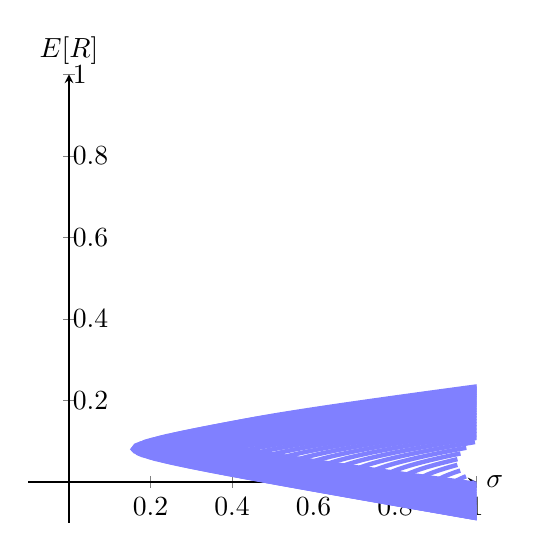
\begin{tikzpicture}
  \begin{axis}[
      xmin=-0.1,
      xmax=1,
      ymin=-0.1,
      ymax=1,
      clip=true,
      unit vector ratio*=1 1 1,
      axis lines=center,
      %grid = major,
      %ytick={-21,-18,...,21},
      %xtick={-21,-18,...,21},
      xlabel=$\sigma$,
      ylabel=${E[R]}$,
      y tick label style={anchor=west},
      every axis y label/.style={at=(current axis.above origin),
        anchor=south},
      every axis x label/.style={at=(current axis.right of origin),anchor=west},
    ]
    \foreach \u in {.1,.2,...,4}{
    \addplot[ultra thick,blue!50!white,variable=\t,domain=-3:3,samples=100] (
            {
              sqrt(.36-.96*\u-.6*\t+.9*\u*\t+.69*\u^2+.4*\t^2)
            },
            {
              .18-.14*\u-.08*\t
            });
            }
            
\end{axis}
\end{tikzpicture}
\end{document}
